\documentclass[10pt,journal,compsoc]{IEEEtran}

\usepackage{cite}
\usepackage{amsmath,amssymb,amsfonts,amsthm,mathtools}
\usepackage{graphicx}
\usepackage{booktabs}
\usepackage{enumitem}
\usepackage{url}
\usepackage{afterpage}
\urlstyle{tt}
\usepackage{tikz}
\usepackage{xr}
\externaldocument[supp-]{build/supplement}
\usetikzlibrary{arrows.meta,positioning,decorations.pathreplacing,automata,calc}
% Unified monochrome figure style for the paper.
% All automata and timing diagrams use white states, black borders and black arrows.
\tikzset{
  fmbracebottom/.style={
    decorate,
    decoration={brace,mirror,amplitude=4pt}
  },
  fmstate/.style={
    circle, draw=black, fill=white, line width=0.6pt,
    minimum size=9mm, inner sep=1pt, font=\small
  },
  fmstatewide/.style={
    rounded rectangle, draw=black, fill=white, line width=0.6pt,
    minimum height=8mm, inner xsep=3pt, inner ysep=1.5pt, font=\small
  },
  fmaccept/.style={fmstate,double,double distance=1.2pt},
  fmerror/.style={fmstate,double,double distance=1.2pt,fill=gray!12},
  fmedge/.style={->,>=Stealth,line width=0.6pt},
  fmlabel/.style={font=\scriptsize,align=center,fill=white,inner sep=1.2pt},
  fminvariant/.style={font=\scriptsize,align=center},
  fmnote/.style={font=\scriptsize,align=center},
  fmtimeline/.style={->,>=Stealth,line width=0.6pt},
  fmevent/.style={circle,draw=black,fill=white,line width=0.6pt,minimum size=4.5mm,inner sep=0.5pt},
  fmreference/.style={fmevent,double,double distance=0.8pt},
  fmguide/.style={densely dashed,line width=0.45pt},
  fmbrace/.style={decorate,decoration={brace,amplitude=4pt},line width=0.5pt}
}


\newtheorem{theorem}{Theorem}[section]
\newtheorem{lemma}[theorem]{Lemma}
\newtheorem{corollary}[theorem]{Corollary}
\newtheorem{proposition}[theorem]{Proposition}
\newtheorem{assumption}[theorem]{Assumption}
\newtheorem{definition}[theorem]{Definition}

\newcommand{\Nat}{\mathbb{N}}
\newcommand{\Real}{\mathbb{R}}
\newcommand{\satM}{\models_{\mathrm{MTL}}}
\newcommand{\satL}{\models_{\mathrm{LTL}}}
\newcommand{\Until}{\mathbin{\mathsf{U}}}
\newcommand{\Release}{\mathbin{\mathsf{R}}}
\newcommand{\hUntil}{\mathbin{\widehat{\mathsf{U}}}}
\newcommand{\hRelease}{\mathbin{\widehat{\mathsf{R}}}}
\newcommand{\Next}{\mathsf{X}}
\newcommand{\Always}{\mathsf{G}}
\newcommand{\Eventually}{\mathsf{F}}
\newcommand{\WeakUntil}{\mathbin{\mathsf{W}}}
\newcommand{\Reset}{\mathsf{rst}}
\newcommand{\Unch}{\mathsf{unch}}
\newcommand{\T}{\mathcal{T}}
\newcommand{\Node}{\mathsf{node}}
\newcommand{\CVal}{\mathsf{val}}
\newcommand{\CReset}{\mathsf{reset}}
\newcommand{\elapsed}{\mathsf{elap}}
\newcommand{\ewbase}{\mathsf{ew\_base}}
\newcommand{\Clock}{\mathit{Clock}}
\newcommand{\runinhead}[1]{\par\smallskip\noindent\textbf{#1}\enspace}
\newcommand{\Rocqid}[1]{{\small\url{#1}}}

\title{A Mechanically Verified Translation of MTL$_{0,\infty}$ into Timed B\"uchi Automata}

\author{Elie Fares, Jean-Paul Bodeveix, Hussain Al-Aqrabi, and Azar Salami%
\thanks{Elie Fares, Hussain Al-Aqrabi, and Azar Salami are with the Higher Colleges of Technology, Sharjah, United Arab Emirates (e-mail: efares@hct.ac.ae; halaqrabi@hct.ac.ae; asalami@hct.ac.ae).}%
\thanks{Jean-Paul Bodeveix is with IRIT, Universit\'e de Toulouse, France (e-mail: bodeveix@irit.fr).}%
}

\begin{document}
\maketitle

\begin{abstract}
We mechanize a soundness and completeness theorem for a specified translation
from pointwise dense-time $\mathrm{MTL}_{0,\infty}$ to event-guarded timed
B\"uchi automata, without location invariants and with existential initial
clock valuations. The
mechanized theorem covers well-formed core formulas: lower and strict upper
bounds are positive, and non-strict upper bounds are nonnegative. We describe
reductions for zero lower bounds and zero strict upper bounds, but do not
mechanize this preprocessing. Ordinary timed operators are expressed through
hatted Until and Release primitives, encoded in clocked LTL, and passed to an
LTL-to-B\"uchi backend satisfying an explicit semantic contract. Relaxation
and reset completion yield a timed B\"uchi automaton. The proof assigns one
clock to each distinct primitive timed subformula, including overlapping
activations. Soundness holds for every clock-consistent reset trace;
completeness constructs a canonical trace using residual obligations. These
arguments establish \texttt{MTL\_\allowbreak{}to\_\allowbreak{}TBA\_\allowbreak{}correct\_\allowbreak{}with}. The result covers strict and non-strict
bounds within the stated core domain; it is not an integrated compiler or a
performance comparison. For the alarm-response instance, we prove in Rocq
that a propositional B\"uchi record manually transcribed from a Spot 2.16
graph has the same language as the translated formula over all propositional
words, then instantiate the timed theorem for that record. This does not
verify Spot or the graph-to-record transcription.
\end{abstract}

\begin{IEEEkeywords}
Metric temporal logic, timed B\"uchi automata, Rocq, formal verification,
clocked LTL, semantic preservation.
\end{IEEEkeywords}

\section{Introduction}
\label{sec:introduction}
Temporal-property translators are part of software verification
infrastructure: changing the timed language can make a downstream verifier
accept a violating execution or reject a valid one. For bounded response,
$\Box(\mathit{req}\Rightarrow\Diamond_{\le d}\mathit{ack})$, overlapping
requests create pending deadlines while reusing one clock for that primitive
timed formula. An incorrect reset at a later request could make an older
deadline appear younger. Table~\ref{tab:overlap-example} illustrates this
general correctness risk; it does not allege a defect in prior tools.

Section~\ref{sec:alarm-example} instantiates this assurance for alarms that
must be handled within three time units. Rocq proves the backend contract for
a manual transcription of a Spot 2.16~\cite{[spot]} graph, applies the timed
theorem, and rejects a fixed violating trace; the graph-to-record link is
outside the proof.

The mathematical translation result substantially predates this paper.
Bulychev et al. prove exact timed-automaton language results for safety and
co-safety fragments; Li et al. state full MTL$_{0,\infty}$ language equality
for their timed-B\"uchi construction (Theorem 12) and prove a best-choice reset
policy language-preserving (Theorem 13)~\cite{[BDLG14],li_spin7}. Those
constructions already use clocks indexed by timed subformulas, obligation
states, and reset/unchanged markers. We claim no new translation algorithm,
clock-allocation principle, or semantic property. The contribution is a
Rocq-checked derivation of the established construction, factored into
clocked-LTL correctness, relaxation, reset completion, and a backend contract.
Its path-indexed induction and canonical-trace completeness make the proof
obligations explicit, but this paper does not establish that these invariants
form a reusable general proof method.

The formal domains also differ: the Rocq model uses real-valued bounds under
the stated well-formedness restrictions, strictly increasing timestamps, and
existential initial clock values; Li et al. use integer bounds, allow equal
timestamps, and start clocks at zero. Thus the present theorem is not a direct
refinement of CASAAL's input/output semantics. The real-bound statement is a
mathematical parameterization, not executable support for arbitrary real
constants.

The factorization is independent of the LTL-to-B\"uchi translator if it
satisfies the contract on all propositional words. Rocq 9.0.1 checks
soundness and completeness for all eight strict and non-strict hatted
primitives, plus relaxation and reset completion, on well-formed Rocq formulas
with real-valued bounds. Zero-bound preprocessing, parsing, backend
integration, output printing, and an executable compiler are outside the
mechanization.

The broader research objective is to derive reusable Event-B refinement
patterns from MTL properties, using TBA as an intermediate representation.
This article establishes the verified MTL-to-TBA stage of that direction;
transforming the resulting automata into Event-B patterns is outside its
present results.

The contributions are verification results for this established
construction:
\begin{itemize}
  \item machine-checked soundness and completeness of the clocked-LTL
        factorization, with soundness for every clock-consistent reset trace
        and completeness through one canonical trace for all formula-keyed
        clocks and repeated activations;
  \item mechanized relaxation and reset completion, composed with an
        explicit language-equivalence contract for the propositional
        backend to obtain the event-guarded TBA theorem;
  \item a concrete alarm-response instance that proves this contract for a
        manual Rocq transcription of a Spot 2.16 graph and rejects a fixed
        violating timed trace.
\end{itemize}

The development includes the results
\texttt{EncodingCorrect\_proved}, \texttt{T\_uses\_every\_clock}, and
\texttt{MTL\_\allowbreak{}to\_\allowbreak{}TBA\_\allowbreak{}correct\_\allowbreak{}with}. The complete arguments for the
canonical policy and its strict-bound cases appear in the supplementary
material. A related unpublished companion manuscript~\cite{fares_bodeveix_tba_optimization}
reports reuse of this Rocq translation
proof and additional TBA optimization and UPPAAL-export results. No stable
public version is available, so those downstream results are outside the
evidence and scope of this paper.

For verification-tool developers, the theorem is a modular reference
contract: a well-formed core Rocq formula and a propositional backend
satisfying Assumption~\ref{ass:backend} yield an event-guarded TBA with the
same timed language under existential initial clock values. A future
implementation can use the Rocq development as a reference; transferring the
guarantee requires separately establishing that its formula mapping, backend,
and output semantics meet these interfaces. Parsing, bound encoding, backend
invocation and validation, export, and adaptation to zero-initialized clocks
are outside the theorem.
The canonical trace is a completeness witness, not a runtime reset policy;
no comparative clock-count, runtime, or automaton-size claim is made. The
Spot script regenerates only the propositional graph, and the worked TBA is
hand-derived; neither is an end-to-end checker run.

\raggedbottom
\afterpage{\flushbottom}
\section{Logic and Semantic Model}
\label{sec:logic}
\subsection{Pointwise MTL$_{0,\infty}$}
\label{sec:mtl}
Let $\Sigma$ be a finite set of actions. Formulas are in negation normal
form and use Boolean operators, next, untimed Until and Release, and timed
Until and Release whose intervals have one endpoint at zero or infinity.
We write a bound as $\sim d$, with $\sim\in\{<,\le,>,\ge\}$. The logic also
contains the hatted operators $\hUntil_{\sim d}$ and
$\hRelease_{\sim d}$. In a hatted operator the current position is skipped
by the logical interval, while its timestamp remains the timing reference.
We use $\widehat{\Box}_{\sim d}\varphi$ as shorthand for
$\bot\hRelease_{\sim d}\varphi$; it requires $\varphi$ at each strictly
future position whose elapsed time from the current position satisfies the
bound.

A timed word is $w=(a_i,t_i)_{i\in\Nat}$, where $a_i\in\Sigma$,
$0\le t_0<t_1<\cdots$, and timestamps diverge. We write
$\elapsed_w(i,j)=t_j-t_i$. For Until, $w,i\satM p\Until_{\sim d}q$
holds when some $j\ge i$ satisfies $q$ and $t_j-t_i\sim d$, with $p$ at
each position in $[i,j)$. For hatted Until, the witness is $j>i$ and $p$
is required on $(i,j)$. Release is the dual universal condition: at every
position in the bounded region, either $q$ holds or $p$ held earlier in the
corresponding interval. Hatted Release excludes the current position from
that region. We use the standard pointwise semantics~\cite{MTLsem}.

For precision, the four bounded clauses used below are:
\begin{align*}
 w,i\satM p\Until_{\sim d}q
 &\Longleftrightarrow \exists j\ge i.\; w,j\satM q\\
 &\quad\land t_j-t_i\sim d\\[-1mm]
 &\quad\land \forall k\in[i,j).\;w,k\satM p,\\
 w,i\satM p\hUntil_{\sim d}q
 &\Longleftrightarrow \exists j>i.\; w,j\satM q\\
 &\quad\land t_j-t_i\sim d\\[-1mm]
 &\quad\land \forall k\in(i,j).\;w,k\satM p,\\
 w,i\satM p\Release_{\sim d}q
 &\Longleftrightarrow \forall j\ge i.\\[-1mm]
 &\quad\Bigl(t_j-t_i\sim d\Rightarrow\\[-1mm]
 &\qquad\Bigl(w,j\satM q\\[-1mm]
 &\qquad\quad\lor \exists k\in[i,j).\;w,k\satM p\Bigr)\Bigr),\\
 w,i\satM p\hRelease_{\sim d}q
 &\Longleftrightarrow \forall j>i.\\[-1mm]
 &\quad\Bigl(t_j-t_i\sim d\Rightarrow\\[-1mm]
 &\qquad\Bigl(w,j\satM q\\[-1mm]
 &\qquad\quad\lor \exists k\in(i,j).\;w,k\satM p\Bigr)\Bigr).
\end{align*}
The index intervals select event positions, whereas $t_j-t_i$ measures
elapsed physical time. Thus, when a bound falls between two events, no event
occurs exactly at that bound, and interval membership is still evaluated at
the event positions.
The strict increase assumption excludes simultaneous events; divergence is
used in the lower-bounded Until fairness argument.

The Rocq development represents action names by natural numbers rather than a
parameterized finite type, and timed words may use any natural-number name.
Each formula mentions finitely many names, so its semantics and generated
labels distinguish actions only by equality or inequality with those names.
Equivalently, the construction operates over the finite quotient induced by
those action tests; this is the finite alphabet used in the mathematical
presentation.

The well-formedness condition requires $d>0$ for every lower bound and strict
upper bound, and $d\ge0$ for a non-strict upper bound. Ordinary timed
operators are definitions in the mechanized core. For upper bounds
$\precsim\in\{\le,<\}$ and lower bounds $\succsim\in\{\ge,>\},$ they are:
\begin{align}
p\Until_{\precsim d}q &\equiv q\lor(p\land(p\hUntil_{\precsim d}q)),\label{eq:derive-ule}\\
p\Until_{\succsim d}q &\equiv p\land(p\hUntil_{\succsim d}q),\label{eq:derive-uge}\\
p\Release_{\precsim d}q &\equiv q\land(p\lor(p\hRelease_{\precsim d}q)),\label{eq:derive-rle}\\
p\Release_{\succsim d}q &\equiv p\lor(p\hRelease_{\succsim d}q).\label{eq:derive-rge}
\end{align}
These definitions separate the current-position case from the strictly future
obligation. Their pointwise semantic compatibility, including the stated
bound hypotheses, is proved in Rocq:
\begin{theorem}[Semantic compatibility of the derived timed operators]
\label{thm:derived-semantic-compatibility}
Under the well-formedness conditions above, Eqs.~\eqref{eq:derive-ule}--
\eqref{eq:derive-rge} agree with the standard pointwise semantics for all
strict and non-strict upper and lower bounds.
\end{theorem}
The identities follow by separating the current-position case from a
strictly future endpoint. For upper Until, a witness at $i$ contributes
$q$; every later witness requires $p$ at $i$ and leaves the hatted
obligation. A lower bound with $d>0$ excludes $i$, so $p$ is required now
and the remaining witness is hatted. The Release identities are the dual
case split: an upper-bound region includes $i$ and therefore requires $q$
there, while a lower-bound region excludes $i$. Strict upper bounds also
require $d>0$, avoiding the degenerate $<0$ case. The eight corresponding
Rocq lemmas are identified in the result map in Supplement~\ref{supp-app:rocq}.
Thus only
the eight hatted timed constructors require primitive translation clauses.
If a source formula has a zero lower bound, strict increase of timestamps
makes every strictly future elapsed time positive. At the hatted level,
$\hUntil_{\ge0}$ and $\hUntil_{>0}$ therefore reduce to
$\Next(p\Until q)$, while $\hRelease_{\ge0}$ and $\hRelease_{>0}$
reduce to $\Next(p\Release q)$. For ordinary operators, the current-position
case must also be simplified: the $\ge0$ cases are the corresponding untimed
Until and Release operators, and the $>0$ cases reduce to
$p\land\Next(p\Until q)$ and $p\lor\Next(p\Release q)$,
respectively. These reductions rely on the paper's strictly increasing event
times and must be applied before encoding a source formula as a Rocq core
formula; the preprocessing itself is not mechanized. A zero strict
upper bound has an empty interval: Until reduces to $\bot$ and Release to
$\top$; strict upper-bound constructors in the core consequently require
$d>0$. For the non-strict upper bound zero, the hatted future operators reduce
to $\hUntil_{\le0}\equiv\bot$ and $\hRelease_{\le0}\equiv\top$, because all
strictly future events have positive elapsed time. The derived ordinary
operators therefore both reduce to their right operand:
$p\Until_{\le0}q\equiv q$ and $p\Release_{\le0}q\equiv q$. These reductions
make the boundary explicit: the mechanized domain excludes zero lower bounds
and zero strict upper bounds, but includes non-strict upper bound zero.

\begin{figure}[t]
\centering
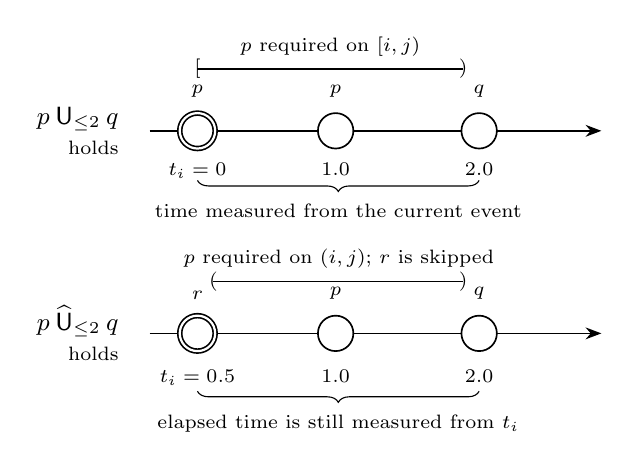
\begin{tikzpicture}[x=1.35cm,y=1.05cm,
  ival/.style={line width=0.5pt},
  ivallab/.style={font=\scriptsize,above=1pt}]
  % Ordinary Until
  \node[anchor=east,font=\small,align=right] at (-0.20,1.30) {$p\Until_{\le 2}q$\\{\scriptsize holds}};
  \draw[fmtimeline] (0,1.30) -- (4.25,1.30);
  \node[fmreference] (u0) at (0.45,1.30) {};
  \node[fmevent] (u1) at (1.75,1.30) {};
  \node[fmevent] (u2) at (3.10,1.30) {};
  \node[above=2pt of u0,font=\scriptsize] {$p$};
  \node[above=2pt of u1,font=\scriptsize] {$p$};
  \node[above=2pt of u2,font=\scriptsize] {$q$};
  \node[below=1.5pt of u0,font=\scriptsize] {$t_i=0$};
  \node[below=1.5pt of u1,font=\scriptsize] {$1.0$};
  \node[below=1.5pt of u2,font=\scriptsize] {$2.0$};
  \draw[ival] (0.45,2.05) -- (2.95,2.05);
  \node[font=\scriptsize] at (0.45,2.05) {$[$};
  \node[font=\scriptsize] at (2.95,2.05) {$)$};
  \node[ivallab] at (1.70,2.05) {$p$ required on $[i,j)$};
  \draw[fmbracebottom] (0.45,0.70) -- node[below=5pt,font=\scriptsize] {time measured from the current event} (3.10,0.70);

  % Hatted Until
  \node[anchor=east,font=\small,align=right] at (-0.20,-1.15) {$p\hUntil_{\le 2}q$\\{\scriptsize holds}};
  \draw[fmtimeline] (0,-1.15) -- (4.25,-1.15);
  \node[fmreference] (h0) at (0.45,-1.15) {};
  \node[fmevent] (h1) at (1.75,-1.15) {};
  \node[fmevent] (h2) at (3.10,-1.15) {};
  \node[above=2pt of h0,font=\scriptsize] {$r$};
  \node[above=2pt of h1,font=\scriptsize] {$p$};
  \node[above=2pt of h2,font=\scriptsize] {$q$};
  \node[below=3pt of h0,font=\scriptsize] {$t_i=0.5$};
  \node[below=3pt of h1,font=\scriptsize] {$1.0$};
  \node[below=3pt of h2,font=\scriptsize] {$2.0$};
  \draw[ival] (0.60,-0.52) -- (2.95,-0.52);
  \node[font=\scriptsize] at (0.60,-0.52) {$($};
  \node[font=\scriptsize] at (2.95,-0.52) {$)$};
  \node[ivallab] at (1.78,-0.52) {$p$ required on $(i,j)$; $r$ is skipped};
  \draw[fmbracebottom] (0.45,-1.85) -- node[below=5pt,font=\scriptsize] {elapsed time is still measured from $t_i$} (3.10,-1.85);
\end{tikzpicture}

\caption{Ordinary and hatted Until. The double circle is the timing reference.
The hatted operator skips the current event logically but measures from its
timestamp.}
\label{fig:hatted-until}
\end{figure}

This distinction is useful for sporadicity: if consecutive occurrences of
$e$ must be separated by at least $\theta$, one may write
$\Box(e\Rightarrow\widehat{\Box}_{<\theta}\neg e)$. The hatted form retains
the triggering event as the time origin; ordinary bounded temporal
operators do not express this particular reference shift directly.
Related pointwise MTL constructions and the CASAAL translation are discussed
in prior work~\cite{ouaknine_worrell_lics05,bouyer_chevalier_markey_fsttcs05,li_spin7,casaal_tool}.

\subsection{Timed B\"uchi Automata}
\label{sec:tba}
The verified target is an event-guarded TBA
$\mathcal A=(L,\ell_0,X,E,\mathit{Acc})$. Here $L$ is a finite set of
locations, $\ell_0$ the initial location, $X$ a finite set of clocks,
$E\subseteq L\times\mathsf{Lab}\times\mathsf{Guard}\times 2^X\times L$
is the set of action-labelled transitions with guards and reset sets, and
$\mathit{Acc}\subseteq L$ the B\"uchi set. A run is a sequence
$(\ell_i,v_i)_{i\ge0}$ starting at $\ell_0$; it follows one transition per
event and visits $\mathit{Acc}$ infinitely often. If the selected edge at
event $i$ is $(\ell_i,\alpha_i,g_i,Z_i,\ell_{i+1})$, then the event action
must satisfy $\alpha_i$ and the valuation $v_i$ must satisfy every guard in
$g_i$. There are no location invariants in this model: timing constraints
are checked at the events of the timed word. This is the TBA record
represented in Rocq; the theorem does not cover a richer invariant-bearing
automaton model without an additional encoding.

Let $v_i$ be the clock valuation tested at event $i$ and
$\Delta_i=t_{i+1}-t_i$. A transition at event $i$ tests $v_i$ before its
reset decision; the next valuation is
\[
v_{i+1}(x)=
\begin{cases}
\Delta_i,&x\in Z_i,\\
v_i(x)+\Delta_i,&\text{otherwise.}
\end{cases}
\]
The initial nonnegative valuation $v_0$ is existentially quantified, as in
the Rocq clock-consistent-extension semantics; standard zero initialization
is not assumed.

\section{Clocked-LTL Translation}
\label{sec:translation}
\subsection{Shared clock identities}
The translation is structural. It maps Boolean and untimed temporal
operators homomorphically and maps each primitive timed subformula to an LTL
formula over an extended alphabet. For each action $a$, the extended
alphabet contains distinct action atoms $\mathsf{LAct}(a)$ and
$\mathsf{LNAct}(a)$, as well as clock-related atoms: clock comparisons
$x\sim d$, a reset atom
$\Reset(x)$, and a preservation atom $\Unch(x)$. Under timed-word
interpretation, the action atoms mean that the current action is $a$ or is
different from $a$, respectively. The atom $\mathsf{LNAct}(a)$ and the
negated literal of $\mathsf{LAct}(a)$ have the same timed-word interpretation,
but remain distinct propositions to the unconstrained LTL backend. The reset
and preservation atoms describe the clock update at the current event. Clock
values are read before the event's reset, matching the guard semantics of a
timed automaton.

For formula $f$, let $\Clock(f)$ be its finite set of distinct primitive
hatted timed subformulas. The clock associated with $F\in\Clock(f)$ is
$x=F$ itself. Clock identity uses structural equality on the Rocq MTL syntax
tree, with bounds compared by equality in $\Real$. Constructor, operands,
comparison, and bound all participate: identical formula values at different
paths share a clock, while semantic equivalence alone does not. No
simplification-based merging is used. The main result proves that this clock
also serves all dynamic activations of its subformula.
The clock count is therefore bounded by the number of distinct primitive
timed subformulas, which is at most the number of timed occurrences in $f$.
If structural subformulas are represented as shared nodes, the translation
can share their LTL encodings as well; this does not remove the usual
worst-case growth of an LTL-to-B\"uchi construction.

This clock-sharing policy is distinct from automaton-state minimization. The
reset trace is chosen for each formula identity as a whole. In particular,
the proof cannot justify the clock bound
by assigning a fresh clock to each activation and subsequently identifying
those clocks: it establishes directly that a single trace of reset decisions
for the formula is sufficient.

\subsection{Eight primitive clauses}
\label{sec:mtlbuchi}
Let $F$ be a primitive hatted formula at path $\pi$, with operands $p,q$.
Write $x=\mathsf{clock\_of}(F)$, $P=\T_{\pi0}(p)$,
$Q=\T_{\pi1}(q)$, and define
$\alpha\WeakUntil\beta=(\alpha\Until\beta)\lor\Always\alpha$.
For upper comparisons $\precsim\in\{\le,<\}$ and lower comparisons
$\succsim\in\{\ge,>\}$, complements are
$\le^{\mathrm c}=>$, $<^{\mathrm c}=\ge$, $\ge^{\mathrm c}=<$, and
$>^{\mathrm c}=\le$. The four clause shapes, each instantiated for its
strict and non-strict bound, give all eight primitive cases:
\begin{align}
\T_\pi(p\hUntil_{\precsim d}q)
 &=\Next\bigl(((x\precsim d)\land\Unch(x)\land P)\nonumber\\
 &\hspace{23mm}\Until((x\precsim d)\land Q)\bigr),\label{eq:t-hule}\\
\T_\pi(p\hUntil_{\succsim d}q)
 &=\Reset(x)\land\Next\bigl((P\Until((x\succsim d)\land(P\Until Q)))\nonumber\\
 &\hspace{23mm}\lor(\Always P\land\Always\Eventually Q)\bigr),\label{eq:t-huge}\\
\T_\pi(p\hRelease_{\precsim d}q)
 &=\Reset(x)\land\Next\bigl(Q\nonumber\\
 &\hspace{23mm}\WeakUntil((x\mathrel{\precsim^{\mathrm c}}d)\lor(P\land Q))\bigr),\label{eq:t-hrle}\\
\T_\pi(p\hRelease_{\succsim d}q)
 &=\Next\bigl(((x\mathrel{\succsim^{\mathrm c}}d)\land\Unch(x))\nonumber\\
 &\hspace{23mm}\WeakUntil((P\Release Q)\lor((x\mathrel{\succsim^{\mathrm c}}d)\land P))\bigr).
 \label{eq:t-hrge}
\end{align}
All clock atoms occur positively. Upper-bounded hatted Until uses strong
Until, matching the mechanized clause: its witness must satisfy $q$ while the
clock remains within the upper bound. On a clock-consistent trace over
divergent time, an infinite continuation cannot keep the preservation guard
true forever. Lower-bounded Until retains its
fairness branch, including $\Always\Eventually Q$, so that eventuality is
not lost. The weak-Until clauses mark the end of bounded Release windows.
Strict comparisons are represented directly; no strict bound is weakened by
adjusting its constant.

The clauses have four distinct temporal roles. For upper-bounded Until, the
clock is tested before any new reset: while its value remains in the allowed
window, $P$ must continue until $Q$ appears. If the bound is passed first, no
bounded witness exists and the strong-Until clause fails. For
lower-bounded Until, a finite path waits for the threshold and then starts
the unbounded $P\Until Q$ obligation. If the threshold is never reached,
the second disjunct requires $P$ at every position and $Q$ infinitely often.
Time divergence is what makes this infinite branch equivalent to a witness
at distance at least $d$.

For upper-bounded Release, the initial $Q$ is required and the weak-until
stops either at the complementary clock comparison or when $P\land Q$
discharges the obligation. For lower-bounded Release, the clock remains
unchanged before the threshold; after that point, the translated obligation
is ordinary Release, with the endpoint alternative covering the transition
into the threshold region. Thus Until clauses use existential witnesses,
whereas Release clauses maintain a universal condition over the bounded
region. The hatted shift is encoded by the outer $\Next$ in every clause;
for restart families, the separate $\Reset(x)$ atom denotes the reference
timestamp at the current position.

\begin{table}[t]
\centering
\caption{Clock comparisons used by each hatted primitive.}
\label{tab:clock-tests}
\footnotesize
\begin{tabular}{@{}lll@{}}
\toprule
Primitive role & Non-strict bound & Strict bound\\
\midrule
$\hUntil_{\precsim d}$ endpoint & $x\le d$ & $x<d$\\
$\hUntil_{\succsim d}$ threshold & $x\ge d$ & $x>d$\\
$\hRelease_{\precsim d}$ window end & $x>d$ & $x\ge d$\\
$\hRelease_{\succsim d}$ pre-threshold & $x<d$ & $x\le d$\\
\bottomrule
\end{tabular}
\end{table}

\subsection{Why hatted operators and shared clocks matter}
The hatted operators preserve the triggering timestamp while moving logical
evaluation to the next event. The same distinction appears in the clocked
encoding: the initial $\Next$ moves the temporal obligation forward, while
the clock retains the reference selected by its reset trace.

For instance, $\Box(e\Rightarrow\widehat{\Box}_{<\theta}\neg e)$ measures
the exclusion window from the triggering event. Prefixing the ordinary
operator with $\bigcirc$ shifts the reference to the next event, while
omitting $\bigcirc$ also constrains the triggering event itself. The three
readings differ on the same timed word, as shown in Fig.~\ref{fig:hat-reference}.
\begin{figure*}[t]
\centering
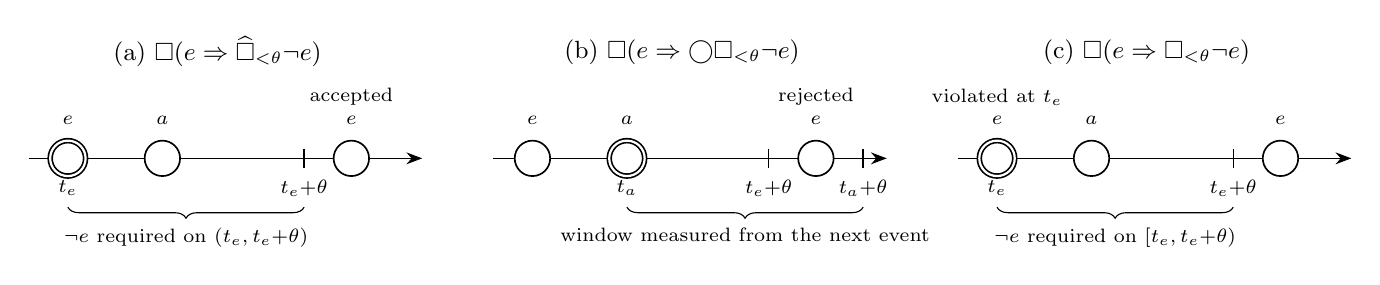
\begin{tikzpicture}[x=1cm,y=1cm,
  tick/.style={line width=0.5pt},
  ticklab/.style={font=\scriptsize,below=1pt},
  verdict/.style={fmnote}]
  % (a) Hatted operator: the intended reading
  \begin{scope}[xshift=0cm]
    \node[font=\small] at (2.4,1.35) {(a) $\Box(e\Rightarrow\widehat{\Box}_{<\theta}\neg e)$};
    \draw[fmtimeline] (0,0) -- (5.0,0);
    \node[fmreference] (a0) at (0.5,0) {};
    \node[fmevent] (a1) at (1.7,0) {};
    \node[fmevent] (a2) at (4.1,0) {};
    \node[above=2pt of a0,font=\scriptsize] {$e$};
    \node[above=2pt of a1,font=\scriptsize] {$a$};
    \node[above=2pt of a2,font=\scriptsize] {$e$};
    \node[verdict] at (4.1,0.78) {accepted};
    \draw[tick] (3.5,0.12) -- (3.5,-0.12) node[ticklab] {$t_e{+}\theta$};
    \node[ticklab] at (0.5,-0.12) {$t_e$};
    \draw[fmbracebottom] (0.5,-0.62) -- node[below=4pt,fmnote] {$\neg e$ required on $(t_e,t_e{+}\theta)$} (3.5,-0.62);
  \end{scope}

  % (b) Replacing the hat by a leading Next
  \begin{scope}[xshift=5.9cm]
    \node[font=\small] at (2.4,1.35) {(b) $\Box(e\Rightarrow\bigcirc\Box_{<\theta}\neg e)$};
    \draw[fmtimeline] (0,0) -- (5.0,0);
    \node[fmevent] (b0) at (0.5,0) {};
    \node[fmreference] (b1) at (1.7,0) {};
    \node[fmevent] (b2) at (4.1,0) {};
    \node[above=2pt of b0,font=\scriptsize] {$e$};
    \node[above=2pt of b1,font=\scriptsize] {$a$};
    \node[above=2pt of b2,font=\scriptsize] {$e$};
    \node[verdict] at (4.1,0.78) {rejected};
    \draw[tick] (3.5,0.12) -- (3.5,-0.12) node[ticklab] {$t_e{+}\theta$};
    \draw[tick] (4.7,0.12) -- (4.7,-0.12) node[ticklab] {$t_a{+}\theta$};
    \node[ticklab] at (1.7,-0.12) {$t_a$};
    \draw[fmbracebottom] (1.7,-0.62) -- node[below=4pt,fmnote] {window measured from the next event} (4.7,-0.62);
  \end{scope}

  % (c) Dropping the Next
  \begin{scope}[xshift=11.8cm]
    \node[font=\small] at (2.4,1.35) {(c) $\Box(e\Rightarrow\Box_{<\theta}\neg e)$};
    \draw[fmtimeline] (0,0) -- (5.0,0);
    \node[fmreference] (c0) at (0.5,0) {};
    \node[fmevent] (c1) at (1.7,0) {};
    \node[fmevent] (c2) at (4.1,0) {};
    \node[above=2pt of c0,font=\scriptsize] {$e$};
    \node[above=2pt of c1,font=\scriptsize] {$a$};
    \node[above=2pt of c2,font=\scriptsize] {$e$};
    \node[verdict] at (0.5,0.78) {violated at $t_e$};
    \draw[tick] (3.5,0.12) -- (3.5,-0.12) node[ticklab] {$t_e{+}\theta$};
    \node[ticklab] at (0.5,-0.12) {$t_e$};
    \draw[fmbracebottom] (0.5,-0.62) -- node[below=4pt,fmnote] {$\neg e$ required on $[t_e,t_e{+}\theta)$} (3.5,-0.62);
  \end{scope}
\end{tikzpicture}

\caption{The hatted sporadicity property and two ordinary-operator
substitutions. A leading next operator shifts the timing reference to the
following event; omitting it includes the triggering event in the window.}
\label{fig:hat-reference}
\end{figure*}

Clock sharing has two layers. First, identical primitive formulas at
different syntax-tree paths share one clock by construction. Second, that
single clock must represent all pending activations. For example, in
$\Box(\mathit{req}\Rightarrow\Diamond_{\le5}\mathit{ack})$, requests at times
0 and 4 overlap. If an acknowledgment occurs at time 6, resetting at the
second request makes its age appear to be two, although the first request's
deadline expired at time 5. The shared-clock construction retains the older
reference and does not accept this word on the basis of the newer request
alone; Table~\ref{tab:overlap-example} records both ages. It is a finite
prefix: every infinite continuation still has the missed deadline for the
request at time 0. More generally, for
any newer request at time $t_k$ between an older activation $t_i$ and a
witness $t_j$, $t_j-t_k\le t_j-t_i$; an endpoint that satisfies the older
upper-bound obligation also satisfies the newer one. The argument depends on
the required $P$ condition holding between activations and the endpoint,
which is exactly what the Until residual records.

\begin{table}[t]
\centering
\caption{Finite prefix showing how a per-request reset can hide an expired
older deadline. Ages are measured immediately before each event; the left
column preserves the oldest request clock, while the right resets at each
request. The deadline is five time units, so no continuation can repair the
miss at time 5.}
\label{tab:overlap-example}
\footnotesize
\begin{tabular}{@{}clccc@{}}
\toprule
Event $i$ & Action & Time $t_i$ & Oldest age & Reset age\\
\midrule
0 & $\mathit{req}$ & 0 & 0 & 0\\
1 & $\mathit{req}$ & 4 & 4 & 4\\
2 & $\mathit{ack}$ & 6 & 6 & 2\\
\bottomrule
\end{tabular}
\end{table}

For the other primitive families, the canonical policy and residual
predicates handle the direction in which restarting or preserving the clock
is required (Supplement~\ref{supp-subsec:timed-completeness}).

\subsection{Canonical reset policy}
\label{subsec:canonical-main}
The encoding quantifies over clock traces. To prove completeness with one
clock for a formula that may be activated arbitrarily often, it is enough to
construct one trace that gives priority to an older activation only while
that activation remains useful. The proof records usefulness by residual
obligations. For upper-bounded Until, the residual says that a witness is
still reachable from the current clock age:
\begin{align*}
\mathsf{URes}_{\precsim}(i,v,d,p,q)\iff
\exists j\ge i.\;&v+\elapsed_w(i,j)\precsim d\\[-1mm]
&\land\ w,j\satM q\\[-1mm]
&\land\ \forall k\in[i,j).\\[-1mm]
&\qquad w,k\satM p,
\end{align*}
where $\precsim$ is either $\le$ or $<$. For lower-bounded Release, the
residual records that every position beyond the threshold is still covered:
\begin{align*}
\mathsf{RRes}_{\ge}(i,v,d,p,q)\iff
\forall j\ge i.\;&d\le v+\elapsed_w(i,j)\Rightarrow\\[-1mm]
&\Bigl(w,j\satM q\\[-1mm]
&\qquad\lor\exists k\in[i,j).\\[-1mm]
&\qquad\qquad w,k\satM p\Bigr),\\
\mathsf{RRes}_{>}(i,v,d,p,q)\iff
\forall j\ge i.\;&d<v+\elapsed_w(i,j)\Rightarrow\\[-1mm]
&\Bigl(w,j\satM q\\[-1mm]
&\qquad\lor\exists k\in[i,j).\\[-1mm]
&\qquad\qquad w,k\satM p\Bigr).
\end{align*}
The strict predicates preserve the strict comparison itself. They are
defined and shifted in the Rocq development (the full definitions and
one-step lemmas are in Supplement~\ref{supp-subsec:timed-completeness}).

The residual predicates are deliberately asymmetric. An upper-Until residual
is existential: one still-reachable endpoint is enough, and that endpoint
can discharge the obligation initiated at the current position. A
lower-Release residual is universal: every position that has entered the
threshold region must satisfy the Release condition. The canonical policy
preserves a clock only when its residual remains true, so clock reuse follows
from the semantic shape of the obligation rather than a syntactic rule such
as “reset on every activation.” This distinction is needed for repeated
activations, but the policy is not part of the generated automaton: it is a
word-dependent witness used only to prove completeness.

For clock $x=F$ with current value $v$, the canonical policy is summarized
in Table~\ref{tab:canonical-policy}. ``Preserve iff'' means that the clock is
not reset exactly under the listed condition; in the remaining cases it is
reset. For the restart families, the stated test is the reset condition.
\begin{table}[t]
\centering
\caption{Canonical reset policy for each timed-operator family.}
\label{tab:canonical-policy}
\footnotesize
\begin{tabular}{@{}p{0.34\columnwidth}p{0.60\columnwidth}@{}}
\toprule
Primitive clock $F$ & Reset decision at position $i$\\
\midrule
$p\hUntil_{\le d}q$ &
Preserve iff $v\le d$, $\mathsf{URes}_{\le}(i,v,d,p,q)$, and
$w,i\not\satM q$.\\
$p\hUntil_{<d}q$ &
Preserve iff $v<d$, $\mathsf{URes}_{<}(i,v,d,p,q)$, and
$w,i\not\satM q$.\\
$p\hUntil_{\ge d}q$, $p\hUntil_{>d}q$,
$p\hRelease_{\le d}q$, $p\hRelease_{<d}q$ &
Reset iff $w,i\satM F$.\\
$p\hRelease_{\ge d}q$ &
Preserve iff $v<d$, $\mathsf{RRes}_{\ge}(i,v,d,p,q)$, and
$w,i\not\satM p$.\\
$p\hRelease_{>d}q$ &
Preserve iff $v\le d$, $\mathsf{RRes}_{>}(i,v,d,p,q)$, and
$w,i\not\satM p$.\\
\bottomrule
\end{tabular}
\end{table}
The canonical extension uses this decision for the formula-keyed clock and
updates its value by
\[
u_0=0,\qquad
u_{i+1}=
\begin{cases}
\Delta_i,&\text{if the policy resets at }i,\\
u_i+\Delta_i,&\text{otherwise.}
\end{cases}
\]
The policy depends on truth in the timed word and, through residuals, on its
future. It is a semantic witness used in the completeness proof, not an
algorithm executed by the translator. Its input is the timed formula itself,
not a syntax-tree path, so identical occurrences share the same reset trace.

The two preservation cases retain an older reference only if the residual
is still true and the current event has not discharged it. A later endpoint
that satisfies the older upper-bounded Until also satisfies newer pending
copies with shorter remaining prefixes. For lower-bounded Release, an old
reference reaches the threshold no later than a newer one; the residual
shift $(i,v)\mapsto(i+1,v+\Delta_i)$ carries the remaining obligation.
Conversely, lower-bounded Until and upper-bounded Release restart when the
current formula is true; their translated continuation keeps any older
obligations represented. The strict cases follow the same organization with
strict residuals and guards.

\subsection{Why one trace suffices for shared activations}
The clock key is the primitive timed formula, not its syntax-tree path or the
dynamic activation that created an obligation. Thus identical subformulas at
different tree positions use the same value and reset trace; the Rocq lemma
\texttt{identical\_\allowbreak{}nodes\_\allowbreak{}share\_\allowbreak{}canonical\_\allowbreak{}trace} proves this equality.
Dynamic activations still impose distinct semantic obligations. The canonical
policy represents them by retaining an older clock reference only while its
residual obligation remains valid.

For an upper-bounded Until, let activations at $i_0\le i_1<j$ share an
endpoint $j$. The older reference gives the stronger deadline constraint,
\[
 t_j-t_{i_1}\le t_j-t_{i_0}\le d.
\]
Its required $p$-prefix contains the suffix required by the newer activation.
Consequently, preserving the older clock while
$\mathsf{URes}_{\precsim}$ holds covers both activations; when the older
residual fails or its endpoint has discharged it, the policy can reset for a
new obligation. This is the invariant used by
\texttt{complete\_UhatLe} and its strict counterpart.

Lower-bounded Release has the dual universal shape. An older reference has at
least the age of a newer one and therefore reaches the lower threshold no
later. The predicate $\mathsf{RRes}$ records whether every position beyond
that threshold remains covered by $q$ or an earlier $p$. While the clock is
preserved, the residual advances by
\[
 (i,v)\longmapsto(i+1,v+\Delta_i),
\]
which is the one-step lemma \texttt{rge\_residual\_shift} used by
\texttt{complete\_RhatGe}. In the dual restart families, a current
activation resets the clock, while the $\Gamma$ branch for lower-bounded
Until and weak-until continuation for upper-bounded Release retain the older
obligations in the LTL formula. The same cases use strict residuals and strict
guards for the strict primitives. The resulting sharing argument is about
semantic obligations, not an assumption that activations are nonoverlapping.

\section{From Clocked LTL to a TBA}
\label{sec:tba-construction}
\subsection{LTL-to-B\"uchi contract}
The backend treats extended atoms as independent propositions. It returns a
propositional B\"uchi automaton whose language is exactly that of the
clocked-LTL formula. The theorem is stated for any such backend, deterministic
or not.
\begin{assumption}[Backend correctness]
\label{ass:backend}
For each formula $F$ and each propositional word $s$ over its atoms,
$\mathsf{PBA\_accepts}(A,s)$ iff $s,0\models F$, where $A$ is the backend
automaton for $F$.
\end{assumption}
This contract ranges over all propositional words, including assignments
that do not correspond to any clock-consistent timed word. That stronger
scope is used by relaxation.

\subsection{Relaxation and reset completion}
\label{sec:reset-completion}
The clocked-LTL formula has positive occurrences of clock-related atoms, so
its propositional language is upward closed in those atoms. In each backend
cube, relaxation deletes negative literals over clock comparisons and
reset/preservation markers and removes irrelevant clock-related atoms;
contradictory cubes are discarded. Action literals are retained as transition
labels. For soundness, first reconstruct an assignment satisfying the
selected original cube and apply the backend contract to that word. Upward
closure then transfers satisfaction to the relaxed word, which can only add
truth on relevant clock-related atoms. The position-by-position
reconstruction is given below.

Each clock belongs to one of two classes. A preservation clock is used with
upper-bound tests and $\Unch(x)$, and a restart clock is used with
lower-bound tests and $\Reset(x)$. Reset completion converts a relaxed cube
into a TBA transition as follows:
\begin{itemize}
  \item reset a preservation clock unless the cube contains $\Unch(x)$;
  \item reset a restart clock exactly when the cube contains $\Reset(x)$;
  \item remove reset and preservation markers, retaining clock tests as the
        transition guard and action literals as its label.
\end{itemize}
The asymmetry is essential. Additional resets only decrease preservation
clock values and hence preserve upper tests. A restart clock can be reset
only when explicitly required, since decreasing it could invalidate a lower
test. The full monotonicity argument is given in
Supplement~\ref{supp-subsec:reset-completion-proof}.

\begin{lemma}[Reset completion]
\label{lem:reset-completion}
For every accepting run of the relaxed backend automaton on a
clock-consistent extension, there is a clock-consistent extension with the
same timed word and initial values whose resets are exactly those prescribed
by reset completion, and the same run is accepting in the resulting TBA.
\end{lemma}

\begin{proposition}[Exactness of relaxation and reset completion]
\label{prop:reset-completion}
Let $f$ be well formed and let $A$ satisfy Assumption~\ref{ass:backend}
for $\T(f)$. The TBA obtained from $A$ by relaxation and reset completion
accepts exactly the timed words $w$ for which $w,0\satM f$, under
existential initial clock values.
\end{proposition}
The relaxation proof uses positivity of the clock atoms in $\T(f)$. A run
of the original B\"uchi automaton remains a run after relaxation. Conversely,
take a run of the relaxed automaton and, at each position, reconstruct an
assignment satisfying the selected original backend cube: make each extended
atom false when its deleted negative literal requires this, and choose values
for removed irrelevant atoms as needed by that cube. The backend contract
then makes the reconstructed word a model of $\T(f)$. It agrees with the
relaxed word on base atoms, while the relaxed word can only add truth on
relevant extended atoms. Upward closure of $\T(f)$ therefore makes the
relaxed word a model as well.
Reset completion then assigns resets monotonically: preservation clocks
become no larger, keeping upper guards true, and restart clocks become no
smaller, keeping lower guards true. Thus the same B\"uchi run remains
accepting. The proof is mechanized as
\texttt{relax\_sound}, \texttt{relax\_complete}, and
\texttt{complete\_complete}.

\runinhead{Acceptance convention.}
The theorem quantifies existentially over the nonnegative clock values at
the first event. This is a property of the accepted timed language; it does
not by itself establish equivalence with an automaton whose clocks must
start at zero. For example, a first transition guarded by $x\ge1$ may be
enabled for one existential initial value and disabled when the first event
is at time zero. The worked example avoids dependence on that value by
resetting its deadline clock on the first transition. The conventional
initialization question is otherwise outside Theorem~\ref{thm:mtl-to-tba-correct}.

\subsection{Worked example: bounded eventuality with an exclusion window}
\label{subsec:worked-translation}
Consider
\[
  f=(\Eventually_{\le5}p)\land(\Always_{<2}\neg p).
\]
It requires $p$ to be false at the origin and until age two, then true by age
five. Figure~\ref{fig:translation-reference-tba} shows a hand-simplified
equivalent one-clock TBA, not the syntax-directed output, which assigns
separate clocks to the two distinct timed subformulas. The steps below show
the clocked-LTL translation and timed reinterpretation.

\begin{figure}[t]
\centering
\resizebox{0.88\columnwidth}{!}{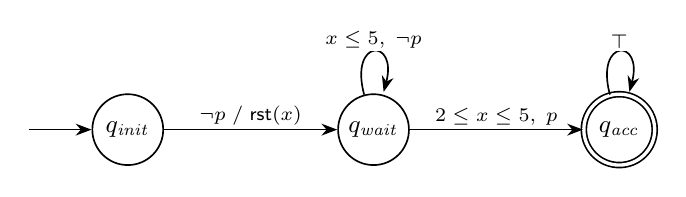
\begin{tikzpicture}[node distance=22mm]
  \node[fmstate] (q0) {$q_{\mathit{init}}$};
  \node[fmstate,right=of q0] (q1) {$q_{\mathit{wait}}$};
  \node[fmaccept,right=of q1] (q2) {$q_{\mathit{acc}}$};
  \draw[fmedge] ([xshift=-8mm]q0.west) -- (q0.west);
  \draw[fmedge] (q0) -- node[fmlabel,above] {$\neg p\;/\;\mathsf{rst}(x)$} (q1);
  \draw[fmedge] (q1) edge[loop above] node[fmlabel] {$x\le5,\;\neg p$} (q1);
  \draw[fmedge] (q1) -- node[fmlabel,above] {$2\le x\le5,\;p$} (q2);
  \draw[fmedge] (q2) edge[loop above] node[fmlabel] {$\top$} (q2);
\end{tikzpicture}
}
\caption{Hand-simplified equivalent event-guarded TBA for $f$. The initial
transition requires $\neg p$ and resets $x$; in the waiting location,
$x\le5$, and acceptance also requires $x\ge2$. Thus $p$ first holds at age
in $[2,5]$.}
\label{fig:translation-reference-tba}
\end{figure}

\begin{enumerate}[label=Step~\arabic*:,leftmargin=*]
\item The formula is in negation normal form. Expanding the derived operators
and applying the timed-operator identities gives
\[
\begin{aligned}
f
 &= (\top\Until_{\le5}p)\land(\bot\Release_{<2}\neg p)\\
 &= \bigl(p\lor(\top\land\top\hUntil_{\le5}p)\bigr)\\
 &\qquad\land\bigl(\neg p\land(\bot\lor\bot\hRelease_{<2}\neg p)\bigr).
\end{aligned}
\]
These current-position cases follow Eqs.~\eqref{eq:derive-ule} and
\eqref{eq:derive-rle}.

\item The two distinct primitive timed subformulas receive clocks $x$ and
$y$, respectively. Their clocked-LTL translation is
\begin{align*}
\Phi_U={}&p\lor\bigl(\top\land\Next\Bigl(
  ((x\le5)\land\Unch(x)\land\top)\Until\\[-1mm]
&\qquad((x\le5)\land p)\Bigr)\bigr),\\[-1mm]
\Phi_R={}&\neg p\land\bigl(\bot\lor(\Reset(y)\land\\[-1mm]
&\qquad\Next(\neg p\WeakUntil((y\ge2)\lor(\bot\land\neg p))))\bigr),\\[-1mm]
\T(f)={}&\Phi_U\land\Phi_R.
\end{align*}
The Until preserves $x$; the Release test $y\ge2$ complements the source
bound $<2$, allowing $p$ from age two.

\item A Spot backend output for $\T(f)$ is shown on the left of
Fig.~\ref{fig:translation-steps45}. Clock guards, reset and preservation
markers, and action atoms are independent propositions to the backend. In
particular, $p=\mathsf{LAct}(p)$ and $\neg p=\mathsf{LNAct}(p)$ are distinct
atoms, while $!p$ is the negated literal of $\mathsf{LAct}(p)$; a backend cube
may contain both $p$ and $\neg p$. Timed reinterpretation imposes action
consistency.

\item Relaxation removes negative literals over extended clock atoms. Reset
completion resets $x$ unless $\Unch(x)$ is present and resets $y$ exactly when
$\Reset(y)$ is present. The right side of Fig.~\ref{fig:translation-steps45}
shows the transitions after marker removal; later optimization removes
unsatisfiable action cubes and simplifies the automaton.
\end{enumerate}

\begin{figure*}[!t]
\centering
\resizebox{\textwidth}{!}{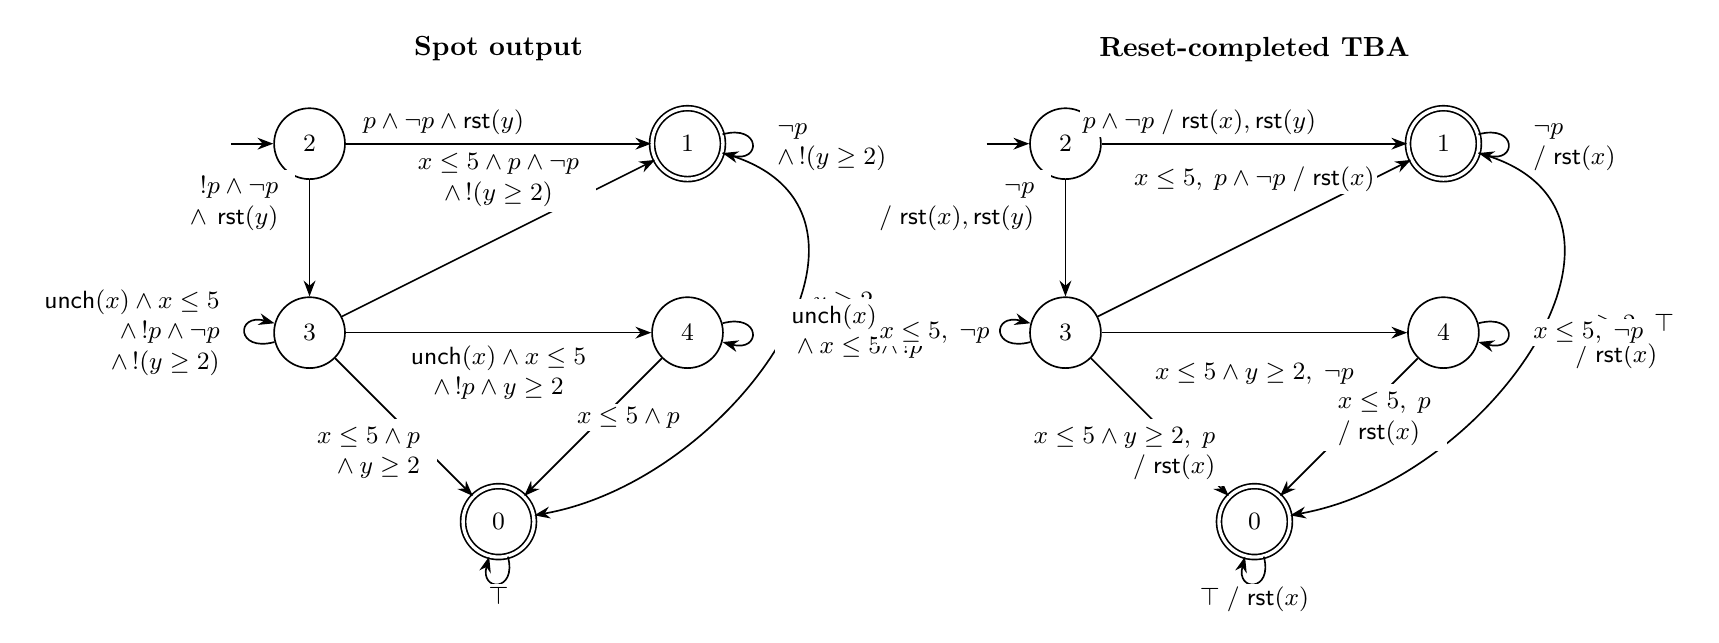
\begin{tikzpicture}[
  x=1cm,y=1cm,
  lab/.style={font=\small,align=center,fill=white,inner sep=1pt}
]
% Left: Spot 2.16 output; state IDs match examples/spot/worked_translation.dot.
\begin{scope}[xshift=0cm]
  \node[fmnote,font=\normalsize\bfseries] at (2.4,6.0) {Spot output};
  \node[fmstate] (l0) at (0.0,4.8) {$2$};
  \node[fmstate] (l1) at (0.0,2.4) {$3$};
  \node[fmaccept] (l2) at (4.8,4.8) {$1$};
  \node[fmstate] (l3) at (4.8,2.4) {$4$};
  \node[fmaccept] (l4) at (2.4,0.0) {$0$};
  \draw[fmedge] (-1.0,4.8) -- (l0);
  \draw[fmedge] (l0) -- (l1);
  \node[lab,anchor=east] at (-0.18,4.05) {$\begin{array}{r}!p\land\neg p\\{}\land\,\mathsf{rst}(y)\end{array}$};
  \draw[fmedge] (l0) -- node[lab,above,pos=.32,yshift=2pt] {$p\land\neg p\land\mathsf{rst}(y)$} (l2);
  \draw[fmedge] (l1) edge[loop left,looseness=5.5] node[lab,left,xshift=-3pt] {$\begin{array}{r}\mathsf{unch}(x)\land x\le5\\{}\land\,!p\land\neg p\\{}\land\,!(y\ge2)\end{array}$} (l1);
  \draw[fmedge] (l1) -- (l2);
  \node[lab] at (2.4,4.35) {$\begin{array}{c}x\le5\land p\land\neg p\\{}\land\,!(y\ge2)\end{array}$};
  \draw[fmedge] (l1) -- (l3);
  \node[lab] at (2.4,1.88) {$\begin{array}{c}\mathsf{unch}(x)\land x\le5\\{}\land\,!p\land y\ge2\end{array}$};
  \draw[fmedge] (l1) -- (l4);
  \node[lab] at (0.75,0.88) {$\begin{array}{r}x\le5\land p\\{}\land y\ge2\end{array}$};
  \draw[fmedge] (l2) edge[loop right,looseness=5.5] node[lab,right,xshift=3pt] {$\begin{array}{l}\neg p\\{}\land\,!(y\ge2)\end{array}$} (l2);
  \draw[fmedge] (l2) to[out=-15,in=10,looseness=1.3] node[lab,right,pos=.42,xshift=4pt] {$y\ge2$} (l4);
  \draw[fmedge] (l3) edge[loop right,looseness=5.5] node[lab,right,xshift=8pt] {$\begin{array}{l}\mathsf{unch}(x)\\{}\land x\le5\land\,!p\end{array}$} (l3);
  \draw[fmedge] (l3) -- (l4);
  \node[lab] at (4.05,1.32) {$x\le5\land p$};
  \draw[fmedge] (l4) edge[loop below,looseness=5] node[lab,below] {$\top$} (l4);
\end{scope}

% Right: relaxation and reset completion, with the same Spot state IDs.
\begin{scope}[xshift=9.6cm]
  \node[fmnote,font=\normalsize\bfseries] at (2.4,6.0) {Reset-completed TBA};
  \node[fmstate] (r0) at (0.0,4.8) {$2$};
  \node[fmstate] (r1) at (0.0,2.4) {$3$};
  \node[fmaccept] (r2) at (4.8,4.8) {$1$};
  \node[fmstate] (r3) at (4.8,2.4) {$4$};
  \node[fmaccept] (r4) at (2.4,0.0) {$0$};
  \draw[fmedge] (-1.0,4.8) -- (r0);
  \draw[fmedge] (r0) -- (r1);
  \node[lab,anchor=east] at (-0.18,4.05) {$\begin{array}{r}\neg p\\/\;\mathsf{rst}(x),\mathsf{rst}(y)\end{array}$};
  \draw[fmedge] (r0) -- node[lab,above,pos=.32,yshift=2pt] {$p\land\neg p\;/\;\mathsf{rst}(x),\mathsf{rst}(y)$} (r2);
  \draw[fmedge] (r1) edge[loop left,looseness=5.5] node[lab,left,xshift=-3pt] {$x\le5,\;\neg p$} (r1);
  \draw[fmedge] (r1) -- (r2);
  \node[lab] at (2.4,4.35) {$x\le5,\;p\land\neg p\;/\;\mathsf{rst}(x)$};
  \draw[fmedge] (r1) -- (r3);
  \node[lab] at (2.4,1.88) {$x\le5\land y\ge2,\;\neg p$};
  \draw[fmedge] (r1) -- (r4);
  \node[lab] at (0.75,0.88) {$\begin{array}{r}x\le5\land y\ge2,\;p\\/\;\mathsf{rst}(x)\end{array}$};
  \draw[fmedge] (r2) edge[loop right,looseness=5.5] node[lab,right,xshift=3pt] {$\begin{array}{l}\neg p\\/\;\mathsf{rst}(x)\end{array}$} (r2);
  \draw[fmedge] (r2) to[out=-15,in=10,looseness=1.3] node[lab,right,pos=.5,xshift=8pt] {$\begin{array}{l}y\ge2,\;\top\\/\;\mathsf{rst}(x)\end{array}$} (r4);
  \draw[fmedge] (r3) edge[loop right,looseness=5.5] node[lab,right,xshift=8pt] {$x\le5,\;\neg p$} (r3);
  \draw[fmedge] (r3) -- (r4);
  \node[lab] at (4.05,1.32) {$\begin{array}{l}x\le5,\;p\\/\;\mathsf{rst}(x)\end{array}$};
  \draw[fmedge] (r4) edge[loop below,looseness=5] node[lab,below] {$\top\;/\;\mathsf{rst}(x)$} (r4);
\end{scope}
\end{tikzpicture}
}
\caption{Spot 2.16 output (redrawn, left) and hand-derived reset-completed
TBA (right; same state IDs). Raw input and DOT are in
\texttt{examples/spot/}. Right-hand edges show guards, actions, and resets;
$\mathsf{rst}(c)$ and $\mathsf{unch}(c)$ mark reset and preservation.}
\label{fig:translation-steps45}
\end{figure*}


\section{Correctness and Clock Bound}
\label{sec:correctness}
\label{sec:encoding-correctness}
An extended word $\rho$ adds, at every position $i$, a value
$\CVal_\rho(i,x)\in\Real_{\ge0}$ and reset decision
$\CReset_\rho(i,x)$ for each $x\in\Clock(f)$. It is clock-consistent when,
for $\Delta_i=t_{i+1}-t_i$,
\begin{equation}
\CVal_\rho(i+1,x)=
\begin{cases}
\Delta_i,&\CReset_\rho(i,x),\\
\CVal_\rho(i,x)+\Delta_i,&\text{otherwise.}
\end{cases}
\label{eq:clock-update}
\end{equation}
The value at position $i$ is the value tested by guards before the reset
decision at that position. Let $\mathsf{same\_base}(\rho,w)$ mean that $w$
is the timed-word projection of $\rho$.

\begin{theorem}[Correctness of the clock encoding]
\label{thm:encoding-correctness}
For every well-formed formula $f$ and timed word $w$,
\begin{align*}
w,0\satM f\quad\Longleftrightarrow\quad
\exists\rho.\;&\mathsf{same\_base}(\rho,w)\\[-1mm]
&\land\ \mathsf{clock\_consistent}(\rho)\\[-1mm]
&\land\ \rho,0\satL\T(f).
\end{align*}
\end{theorem}
The existential quantifier over $\rho$ is taken jointly over all distinct
primitive timed subformulas. Soundness does not rely on choosing the canonical trace:
each clock may follow any reset pattern allowed by the encoding, provided its
value recurrence is respected. Completeness is the more delicate half
because all activations that share a formula-keyed clock must be served
simultaneously. The proof constructs the clock traces in parallel, using the
residual predicates only for the preservation families and the direct
restart rule for the remaining families.
This result is the Rocq theorem \texttt{EncodingCorrect\_proved}. Its
soundness direction holds for any clock-consistent reset trace. Completeness
constructs one canonical trace for all clocks together. The detailed
induction, including the strict-bound arithmetic, is in
Supplement~\ref{supp-sec:supp-proof}.

\begin{corollary}[One clock per distinct primitive timed subformula]
\label{cor:one-clock-formula}
All occurrences of the same primitive timed subformula use the same logical
clock. The encoding uses exactly the clocks in $\Clock(f)$, hence at most
one clock per distinct primitive timed subformula, independently of the
number of syntax-tree occurrences or run-time activations.
\end{corollary}
\begin{proof}
Every clock in $\T(f)$ is indexed by an element of $\Clock(f)$, and
\texttt{T\_uses\_every\_clock} proves that every such element occurs in
$\T(f)$. A single extension assigns one value and reset trace to each
element of $\Clock(f)$. Theorem~\ref{thm:encoding-correctness} proves that
the canonical trace suffices for every pending activation of that formula.
\end{proof}

Define $\mathsf{compile\_with}(A)$ by applying relaxation and reset
completion to backend automaton $A$. Timed acceptance is existential over
clock-consistent extensions of the timed word and requires that reset
decisions agree with the reset sets along an accepting run.
\begin{theorem}[MTL-to-TBA correctness]
\label{thm:mtl-to-tba-correct}
\label{cor:mtl-tba-correct}
For every well-formed $f$, backend automaton $A$ satisfying
Assumption~\ref{ass:backend}, and timed word $w$,
\[
w,0\satM f\quad\Longleftrightarrow\quad
\mathsf{TBA\_accepts}(\mathsf{compile\_with}(A),w).
\]
In Rocq this is \texttt{MTL\_\allowbreak{}to\_\allowbreak{}TBA\_\allowbreak{}correct\_\allowbreak{}with}; the backend
correctness is an explicit hypothesis, not a project-specific axiom.
\end{theorem}
\begin{proof}
Combine Theorem~\ref{thm:encoding-correctness} with
Proposition~\ref{prop:reset-completion}. The forward direction uses the
canonical extension and reset-completion lemma; the reverse direction uses
upward closure under relaxation, the backend contract, and clock-encoding
soundness.
\end{proof}

\subsection{Semantic and arithmetic proof facts}
\label{subsec:main-proof-facts}
The proof uses the standard LTL expansions of always, eventually, and weak
Until. For every LTL formula $A$ and position $i$,
\begin{align}
\rho,i\satL \Always A &\Longleftrightarrow
  \forall j\ge i,\;\rho,j\satL A,\nonumber\\
\rho,i\satL \Eventually A &\Longleftrightarrow
  \exists j\ge i,\;\rho,j\satL A,\nonumber\\
\rho,i\satL \Always\Eventually A &\Longleftrightarrow
  \forall n\ge i\;\exists j\ge n,\;\rho,j\satL A,\label{eq:main-sem-GF}\\
\rho,i\satL A\WeakUntil B &\Longleftrightarrow
  \Bigl(\exists j\ge i.\;\rho,j\satL B\\[-1mm]
  &\qquad\land\forall k\in[i,j).\;\rho,k\satL A\Bigr)\nonumber\\[-1mm]
  &\qquad\lor\forall j\ge i.\;\rho,j\satL A.\nonumber
\end{align}
These are the Rocq lemmas \texttt{LG\_semantics},
\texttt{LF\_semantics}, \texttt{LGF\_semantics}, and
\texttt{LW\_semantics}. Time divergence also gives a future $B$ position at
any required physical distance when $\Always\Eventually B$ holds
(\texttt{GF\_far}), which supplies the witness in the fairness branch of
lower-bounded Until.

Clock consistency converts guards into elapsed-time bounds.
\begin{lemma}[Accumulation under preservation]
\label{lem:clock-accumulation}
If $x$ is not reset in $[i,j)$, then
\[
\CVal_\rho(j,x)=\CVal_\rho(i,x)+\elapsed_w(i,j).
\]
\end{lemma}
Since clock values are nonnegative, $\elapsed_w(i,j)\le\CVal_\rho(j,x)$.
Thus an upper guard $x\le d$ at $j$ entails
\begin{equation}
\elapsed_w(i,j)\le d.
\label{eq:upper-clock}
\end{equation}
An upper guard $x<d$ gives the strict version.

\begin{lemma}[Clock value after a reset]
\label{lem:clock-after-reset}
If $x$ is reset at $i$ and $j\ge i+1$, then
$\CVal_\rho(j,x)\le\elapsed_w(i,j)$. If it is not reset again before $j$,
equality holds.
\end{lemma}
A later reset only makes the clock younger. Hence a lower guard gives
\begin{equation}
x\ge d\quad\Longrightarrow\quad
d\le\CVal_\rho(j,x)\le\elapsed_w(i,j),
\label{eq:lower-clock}
\end{equation}
and $x>d$ entails a strict lower bound. The Rocq lemmas are
\Rocqid{preserve_accumulate},
\Rocqid{after_reset_value_le_elapsed}, and
\Rocqid{reset_preserve_value_eq_elapsed}.

\subsection{Strict-bound cases}
\label{subsec:main-strict-bounds}
The eight hatted constructors are the primitive proof families. Ordinary
timed operators have already been reduced by
Eqs.~\eqref{eq:derive-ule}--\eqref{eq:derive-rge}. Strict comparisons remain
strict through each translation and proof case. In particular, preservation
gives $\elapsed_w(i,j)\le\CVal_\rho(j,x)$, so $x<d$ implies
$\elapsed_w(i,j)<d$. After a reset,
$\CVal_\rho(j,x)\le\elapsed_w(i,j)$, so $x>d$ implies
$\elapsed_w(i,j)>d$.

The fairness branch of $\hUntil_{>d}$ needs one additional step. Time
divergence gives a future $q$ at distance at least $d$ from position $i+1$;
strict timestamp increase gives $t_{i+1}>t_i$. The same witness is therefore
at distance strictly greater than $d$ from $i$. This is the Rocq lemma
\texttt{sound\_UhatGt}.

\subsection{Mechanization Challenges and Proof Architecture}
\label{subsec:mechanization-challenges}
The proof separates soundness from completeness. For soundness, every
clock-consistent reset trace satisfying the clocked-LTL encoding implies MTL
satisfaction. For completeness, each timed word satisfying the MTL formula
admits an existential canonical clock-consistent trace satisfying the
encoding. Relaxation and reset completion then preserve the timed language.
The following points identify the Rocq invariants used for these obligations.

\runinhead{A. Occurrence-indexed induction with formula-keyed clocks.}
The recursive translation is written as $\T_\pi(f)$: its recursive calls
extend the syntax-tree path $\pi$. Clock identity, however, depends on the
exact primitive-formula syntax and is independent of that path: syntactically
different primitive formulas have different keys, while identical formulas
at distinct positions in the tree use the same clock value and reset trace.
A root-only induction statement does not expose the
child-occurrence facts needed at each recursive call while retaining that
root-wide clock identity. The development proves
\Rocqid{canonical_encoding_all}, whose induction statement ranges over
every path $\pi$ for which $\Node(\mathit{root},\pi)=f$. The lookup lemmas
\Rocqid{node_at_left_binary} and \Rocqid{node_at_right_binary}
establish the child paths; \Rocqid{identical_nodes_share_clock} and
\Rocqid{identical_nodes_share_canonical_trace} show that equal
formula keys denote one clock and one trace. This remains structural
induction on $f$, with a stronger path-indexed invariant. The lemmas
\Rocqid{T_at_uses_clocks} and \Rocqid{T_uses_every_clock} also show
that the encoding uses exactly the formula-indexed clock set.

\runinhead{B. Completeness with repeated activations.}
One clock must support every activation of a primitive formula, including
activations that overlap and have different remaining deadlines. Completeness
cannot choose a separate clock trace for each activation; it must construct a
single clock-consistent extension that satisfies all of them. For upper-bounded
Until, \Rocqid{ule_residual} (and its strict counterpart
\Rocqid{ult_residual}) records a still-available witness, its remaining
deadline, and the required $p$-prefix. The preservation rule retains the
older reference only while this residual remains true and $q$ has not already
discharged it. That reference imposes the stronger deadline and prefix
constraint, so it also covers newer pending activations. For lower-bounded
Release, \Rocqid{rge_residual} and \Rocqid{rgt_residual} record the universal
obligation beyond the threshold: each such position must satisfy $q$ or have
an earlier $p$ that discharges the obligation. The shift lemmas
\Rocqid{rge_residual_shift} and \Rocqid{rgt_residual_shift} carry this
condition across an event while the clock is preserved. These are the two
preservation families. Lower-bounded Until and upper-bounded Release instead
restart their clock at a satisfying activation; their translated temporal
continuations retain older obligations. The eight completeness lemmas in
Table~\ref{tab:primitive-proof-lemmas} prove these cases, including their
strict variants.

\runinhead{C. Relaxation and reset completion.}
The propositional backend treats clock tests and reset markers as independent
atoms, so its language contract applies even to words that are not valuations
of any clock-consistent timed trace. Relaxation deletes negative literals
over these extended atoms. To recover a model of the clocked-LTL formula, the
proof rebuilds at each position an assignment satisfying the original backend cube, then
uses positivity of the translated formula to show that adding truth to
extended atoms preserves satisfaction. The Rocq lemmas \Rocqid{psat_mono},
\Rocqid{relax_sound}, and \Rocqid{relax_complete} formalize this argument.
Reset completion is a separate obligation because it fixes the actual reset
set of each TBA edge. It may reset a preservation clock more often, producing
no larger values and preserving upper-bound tests; for a restart clock it
resets only when the cube requires it, producing no smaller values and
preserving lower-bound tests. The local and run-level arguments are captured
by \Rocqid{complete_trans_sound}, \Rocqid{complete_sound}, and
\Rocqid{complete_complete}. The proof does not assume that the backend
understands clocks.

\runinhead{D. Strict temporal boundaries.}
The strict constructors require proof obligations with $<$ and $>$ preserved
through both the residual predicates and the clock-value inequalities. The
strict residuals \Rocqid{ult_residual} and \Rocqid{rgt_residual}, together
with \Rocqid{preserve_strict_upper_guard_sound} and
\Rocqid{reset_strict_lower_guard_sound}, keep those boundaries explicit.
One additional argument occurs in the fairness branch of $\hUntil_{>d}$:
time divergence and \Rocqid{GF_far} yield a $q$ at distance at least $d$
from position $i+1$, and strict timestamp increase gives $t_{i+1}>t_i$,
making the same witness strictly more than $d$ after $i$
(\Rocqid{sound_UhatGt}). The proof works
over real-valued bounds in the stated well-formed domain; zero-bound
preprocessing remains outside the mechanization. Table~\ref{tab:primitive-proof-lemmas}
lists the separate proof pair for each of the eight cases. These invariants
document the work needed to mechanize this translation; formula/residual and
reset-marker constructions have close mathematical precedents. The current
development does not demonstrate proof reuse for another translator or
extract an executable translation tool.

\begingroup
\raggedright
\runinhead{Artifact Availability.}
The public repository at
\url{https://github.com/efares1/coq-verified-mtl-to-tba} hosts the Rocq
development, alarm-response instance, Spot examples, and reproduction
instructions. This revision adds executable checks for the saved DOT/record
correspondence and a reset-risk scenario; these are included in the local
submission candidate but have not been published to GitHub. The checks are not
verified components. Rocq proves the record's language contract, while Spot
and the DOT-to-record link remain outside the proof. The GitHub URL is mutable;
an immutable identifier for the exact snapshot should be inserted after the
release is approved and publicly archived. This is not an executable compiler.
\par
\endgroup
% SUBMISSION INSERTION: cite the immutable public release/DOI for the exact
% artifact snapshot here once approved and published. The local release
% candidate is not a public artifact.

\begin{table}[t]
\centering
\caption{Rocq lemmas for the primitive timed proof cases. Each strict and
non-strict comparison has its own row.}
\label{tab:primitive-proof-lemmas}
\footnotesize
\begin{tabular}{@{}lll@{}}
\toprule
Primitive family & Soundness & Canonical completeness\\
\midrule
$\hUntil_{\le d}$ & \texttt{sound\_UhatLe} & \texttt{complete\_UhatLe}\\
$\hUntil_{\ge d}$ & \texttt{sound\_UhatGe} & \texttt{complete\_UhatGe}\\
$\hRelease_{\le d}$ & \texttt{sound\_RhatLe} & \texttt{complete\_RhatLe}\\
$\hRelease_{\ge d}$ & \texttt{sound\_RhatGe} & \texttt{complete\_RhatGe}\\
$\hUntil_{<d}$ & \texttt{sound\_UhatLt} & \texttt{complete\_UhatLt}\\
$\hUntil_{>d}$ & \texttt{sound\_UhatGt} & \texttt{complete\_UhatGt}\\
$\hRelease_{<d}$ & \texttt{sound\_RhatLt} & \texttt{complete\_RhatLt}\\
$\hRelease_{>d}$ & \texttt{sound\_RhatGt} & \texttt{complete\_RhatGt}\\
\bottomrule
\end{tabular}
\end{table}

\Rocqid{EncodingCorrect_proved} collects the local cases;
\Rocqid{MTL_to_TBA_correct_with} composes them under the explicit backend
contract. The supplement gives the detailed proofs and theorem composition.

\runinhead{What the mechanization assumes.}
The proof boundary is summarized in Table~\ref{tab:proof-boundary}. In
particular, the correctness of the untimed backend is an explicit
proposition-level assumption; the timed proof does not depend on Spot or on
determinism. The theorem \Rocqid{MTL_to_TBA_correct_with} accepts backend
language equivalence as an explicit argument. The convenience theorem
\Rocqid{MTL_to_TBA_correct} instead uses the project axiom
\Rocqid{LTL_TO_BUCHI_CORRECT}. The audit in
\Rocqid{proof/ASSUMPTIONS.txt} records the standard Rocq library assumptions
for real-number reasoning, functional extensionality, description, and
classical logic. These are separate from the backend contract and the
convenience theorem's project axiom. More precisely, the audit for
\Rocqid{EncodingCorrect_proved} lists only standard/classical assumptions;
\Rocqid{MTL_to_TBA_correct_with} takes backend equivalence as an explicit
premise; \Rocqid{MTL_to_TBA_correct} additionally depends on
\Rocqid{LTL_TO_BUCHI_CORRECT}; and the alarm theorem has standard assumptions
because its record contract is proved separately. Parsing, backend
invocation, and output printing are outside this theorem.
\begin{table}[t]
\centering
\caption{Scope of the mechanized translation theorem.}
\label{tab:proof-boundary}
\footnotesize
\begin{tabular}{@{}p{0.30\columnwidth}p{0.63\columnwidth}@{}}
\toprule
Pipeline stage & Assurance boundary and software consequence\\
\midrule
Formula front end & Input is a well-formed Rocq formula; parsing and finite bound encoding are outside the theorem.\\
Timed encoding & Rocq proves clocked-LTL equivalence using one clock per distinct primitive timed formula.\\
Propositional backend & The generic theorem assumes the backend contract; Rocq proves it for a manual transcription of one Spot 2.16 graph.\\
Graph correspondence & Python checks the saved DOT/record states, acceptance, and guards; importer correctness and Spot remain unverified.\\
TBA construction & Rocq proves relaxation and reset completion; output has event guards and no location invariants.\\
Model-checker adapter & Initial clock values are existential; zero initialization and export adapters are outside the theorem.\\
Integration & No end-to-end translator or timed-checker run; scripts demonstrate one graph correspondence and an illustrative reset fault.\\
\bottomrule
\end{tabular}
\end{table}

\subsection{Alarm-response proof instance}
\label{sec:alarm-example}
Consider $f_{\mathit{alarm}}=\mathsf{G}(\mathit{alarm}\Rightarrow
\Diamond_{\le 3}\mathit{handled})$, meaning every alarm must be handled within
three time units. In
\Rocqid{proof/OverlappingResponse_Example.v}, the formula is
\texttt{MR MFalse (MOr (MNotAtom ALARM) (MUle 3 MTrue (MAtom HANDLED)))},
where \texttt{ALARM} and \texttt{HANDLED} are actions 1 and 2. Rocq checks
that it is well formed and has one primitive timed subformula,
$\widehat{\mathsf{U}}_{\le 3}\,\top\,\mathit{handled}$, whose obligations
share clock $x$. Abbreviate $\mathsf{LNAct}(\mathit{alarm})$ by $N$,
$\mathsf{LAct}(\mathit{handled})$ by $H$, $x\le3$ by $C$, and
$\mathsf{LUnch}(x)$ by $U$. Spot receives the exact clocked-LTL formula
\[
\mathsf{G}\bigl(N\lor H\lor \Next((C\land U)\Until(C\land H))\bigr).
\]
Spot 2.16's input and output are saved in
\Rocqid{examples/spot/alarm_response_backend.ltl} and
\Rocqid{examples/spot/alarm_response_backend.dot}. The generated graph has
initial state 0, accepting set $\{0,1\}$, and these transitions:
\[
\begin{array}{c|c|l}
\text{source}&\text{target}&\text{label}\\ \hline
0&0&H\lor N\\
0&1&\neg H\land\neg N\\
1&0&C\land H\\
1&2&C\land\neg H\land U\\
2&0&C\land H\\
2&2&C\land\neg H\land U
\end{array}
\]
The graph is manually transcribed as
\Rocqid{alarm_response_spot_backend}; Rocq splits the disjunctive
self-loop into two cubes. Lemma
\Rocqid{alarm_response_T_eq} matches its input to the Rocq translation;
\Rocqid{alarm_response_spot_backend_contract} proves that the transcribed
automaton has exactly that LTL language on all propositional words. This
discharges the backend premise for this instance. The regeneration script
requires \texttt{ltl2tgba --version} to report Spot 2.16.

The resulting concrete TBA is
\Rocqid{alarm_response_spot_tba}. Theorem
\Rocqid{alarm_response_spot_tba_correct} instantiates
Theorem~\ref{thm:mtl-to-tba-correct} and proves that it accepts exactly the
timed words satisfying $f_{\mathit{alarm}}$. Its compiled transition listing
is included in the supplementary material for inspection.

For the fixed infinite trace with alarms at times 0 and 2 and a handled event
at time 4, \Rocqid{alarm_response_trace_violates} proves that the first
alarm misses its deadline. Corollary
\Rocqid{alarm_response_trace_rejected_by_spot_tba} proves that this
TBA rejects it. The graph regenerates with the Spot 2.16 command in
\texttt{examples/spot/regenerate.sh}. No graph importer, timed model checker,
or TBA export is verified or run. The repository's Python consistency check
matches the saved graph and Rocq record up to state renaming, including all
guards; mutation self-tests reject a changed guard and accepting set. A
separate illustrative scenario shows how an intentionally incorrect reset at
each request can accept this trace. These executable checks do not establish
universal correctness or make a claim about CASAAL.

\section{Related Work}
\label{sec:related}
\begin{table*}[!t]
\centering
\caption{Theorem and evidence comparison with the closest MTL$_{0,\infty}$
automata constructions. Bulychev et al. prove exactness for safety/co-safety;
Li et al. state full-fragment language equality. No row ranks efficiency.}
\label{tab:prior-construction-comparison}
\small
\setlength{\tabcolsep}{3pt}
\begin{tabular}{@{}p{0.12\textwidth}p{0.22\textwidth}p{0.34\textwidth}p{0.27\textwidth}@{}}
\toprule
Work & Semantic scope & Existing correctness and construction & Mechanization and implementation evidence\\
\midrule
Bulychev~\cite{[BDLG14]} & Pointwise non-Zeno infinite words; integer bounds, all four comparisons, nondecreasing timestamps. & Theorems 1--2 prove exact automaton languages for safety/co-safety. The construction already uses timed-subformula clocks, obligations, and reset/unchanged markers. & Mathematical proofs and controller-synthesis tooling; no mechanized full-fragment TBA theorem.\\
Li et al.~\cite{li_spin7} & Full MTL$_{0,\infty}$; pointwise non-Zeno words, integer bounds, all four comparisons, nondecreasing timestamps, zero initial clocks. & Theorem 12 states exact language equality for the timed-B\"uchi construction; Theorem 13 proves best-choice resets language-preserving. & CASAAL implements the workflow and deterministic approximations~\cite{casaal_tool}; the proof is mathematical.\\
This paper & Well-formed Rocq formulas with real bounds, strictly increasing timestamps, existential nonnegative initial clocks. & \texttt{EncodingCorrect\_proved} proves clocked-LTL equivalence for all eight primitive cases; TBA composition is conditional on backend equivalence. & Rocq-checked proof and one proved contract for a manual Spot transcription; no executable MTL compiler or performance comparison.\\
\bottomrule
\end{tabular}
\end{table*}

Pointwise MTL has extensive decidability and expressiveness results
\cite{[RK90],[RTH96],MTLsem,ouaknine_worrell_lics05,
bouyer_chevalier_markey_fsttcs05}. Unrestricted dense-time MTL has no general
effective translation to finite ordinary timed automata; bounded-variability
and alternating-automaton results have different scopes
\cite{nickovic_piterman_formats10,[BM14]}. MTL$_{0,\infty}$ retains common
response and separation properties~\cite{[RTH96],[BDLG14]}. Our hatted
operators make the timing reference explicit in the logic and proof.

\runinhead{Translations of timed logics.}
As Table~\ref{tab:prior-construction-comparison} shows, the full-fragment
language-equivalence theorem already appears in Li et al. The overlap trace
illustrates a generic reset risk, not a defect in prior tools; we do not claim
their constructions or proofs omit overlapping obligations. Our result is a
machine-checked derivation for a different formal model and proof boundary,
not a new language-correctness property or reset algorithm.

MITL translations use temporal testers, automata networks, or one-clock
alternating automata~\cite{maler_mitl_to_ta,
ferrere2019_realtimelogic_to_ta,[BM14]}; MightyL and MITL2Timed provide
UPPAAL-oriented tools for that distinct logic
\cite{mightyl_paper17,mitl2timed_github}. Obligation-merging techniques are
related, while our one-sided residual predicates support the checked
completeness proof.

\runinhead{Clocked temporal logic and subformula clocks.}
CLTLoc adds clock comparisons and reset predicates to LTL and has been used to
encode metric logics~\cite{bersani_cltloc}. Our similar propositional
vocabulary is an automaton-synthesis intermediate: the backend treats clock
tests and reset markers as propositions. Positivity gives upward closure, and
reset completion restores timed meaning; hence the explicit relaxation proof.

Event-clock logics associate clocks with subformulas to measure time since or
until events~\cite{afh_eventclock_tcs99,
raskin_schobbens_jalc99,nickovic_piterman_formats10}. Formula-indexed clocks
are established; our proof checks that one clock per distinct timed formula
preserves language across repeated activations and all strict and non-strict
cases (Section~\ref{subsec:mechanization-challenges}).

\runinhead{Recent automata-based real-time verification.}
Recent neighboring work addresses different settings: an improved one-clock
alternating MTL automaton for finite timed words with clock deactivation and
zone analysis~\cite{bouyer_srivathsan_vishwanath_fossacs25}; and TEMPORA's
pointwise MITL model checking with past and future modalities
~\cite{akshay_et_al_tempora26}. These do not
translate our MTL$_{0,\infty}$ fragment to infinite-word TBAs.
Ho et al.'s MightyPPL translates pointwise MITL with past and Pnueli
modalities over finite and infinite timed words; it gives mathematical
construction results and proof sketches alongside a complete implementation
whose testers sequentialize overlapping obligations
\cite{mightyppl_tacas26}. The QEST+FORMATS follow-up implements existentially
punctual MTLPPL~\cite{mightyppl_qest26,mightyppl_qest_arxiv26}. Its term
\emph{one-sided MTL} denotes the subfragment without past or Pnueli, whereas
here it describes interval shapes $[0,d]$ and $[d,\infty)$. Any syntactic
containment comparison is limited to conventional source formulas after
zero-bound reduction and with integer bounds; it excludes hatted AST
constructors. The QEST fragment also permits punctual and non-one-sided
intervals in its stated positions. Its punctual-response example does not
imply support for unrestricted punctual MTL; differing bounds and timed-word
conventions preclude a shared-input semantic comparison.

These tools address different fragments or output models; this paper neither
re-verifies them nor makes a shared-input, coverage, clock-count, or
performance comparison. The Rocq development is not integrated with CASAAL,
MightyPPL, or another checker.

\runinhead{Mechanized translations and trusted backends.}
Mechanized work verifies LTL-to-B\"uchi translations and model checkers
\cite{schimpf_tphols09,cava_cav13,ltl_to_gba_afp,seidl_sickert_afp19}.
Wang et al. verify an MLTL-to-regular-expression transformation, export
executable code, and compare it with existing implementations
\cite{wang_mltl_tacas25}. For metric logics, Roohi and Viswanathan used PVS
to correct an unsound release semantics in prior MITL decision procedures
and prove supporting results for an adapted timed-automata construction
under continuous-time signal semantics~\cite{roohi_viswanathan_vmcai18};
Coq-based quantitative MTL monitoring addresses another task
\cite{chattopadhyay_mamouras_rv20}. These targets differ from our pointwise
infinite-word TBA theorem, but set precedents for proof-connected tools and
for mechanization that changes a known result. Here the backend remains an
explicit contract: no LTL translator is integrated or extracted, and Spot
is not verified.

\runinhead{Event-B refinement patterns.}
Our work on Event-B patterns addresses their generation and refinement,
including DSL-based pattern generation~\cite{fares_abz23}, patterns using
weakest-precondition calculus~\cite{fares_facs24}, and pattern-based
development using predicate transformers~\cite{fares_scp27}. These works
provide the Event-B pattern-generation context for our broader objective:
given an MTL property, use its TBA translation as the input to a downstream
Event-B pattern-generation step. The present paper establishes the MTL-to-TBA
stage only. It gives no TBA-to-Event-B transformation or correctness result
for generated Event-B patterns.

\section{Conclusion}
Under an explicit backend contract, we mechanize semantic preservation from
well-formed core $\mathrm{MTL}_{0,\infty}$ formulas to event-guarded timed
B\"uchi automata with existential initial clocks. Clocked-LTL factorization
and reset completion preserve the timed language with one clock per
syntactically distinct primitive timed subformula.

Related constructions already have mathematical language-correctness
results, including Li et al.'s full-fragment MTL$_{0,\infty}$-to-TBA result.
This paper contributes a Rocq-checked derivation for its
real-bound, strictly increasing-time model and explicit backend boundary.
The occurrence-indexed invariant and canonical reset-trace argument support
that proof but are not shown to be reusable beyond this development. No new
clock architecture, reset algorithm, or comparative efficiency result is
established.

For the alarm, Rocq proves the backend contract for a manual Spot 2.16
transcription and instantiates the timed theorem to reject a fixed violating
trace. An executable graph check improves auditability of that transcription,
but its parser is unverified; no integrated translator, timed checker, or
performance study is provided. An immutable public artifact identifier must
be added before final submission.

\bibliographystyle{IEEEtran}
\bibliography{references}
\end{document}
